\begin{abstract}
How quickly does a language model acquire toxic behavior, and how much clean-data training is needed to reduce it? We study this question in a controlled GPT-2-small setting using four proportions of hate-labeled tweets mixed with WikiText-103, three data seeds, and one subsequent epoch of clean training. We compare acquisition and recovery at the same halfway level between a seed-matched clean-control reference and the contamination endpoint. Monotone smoothing and explicit crossing intervals yield per-run asymmetry lower bounds above one, although two of twelve recovery trajectories remain censored at 5,900 recorded steps. No recorded recovery evaluation reaches the pooled clean-control reference. Re-evaluating final checkpoints on generated continuations alone preserves the paired contamination--recovery difference and leaves recovered models at roughly four times the mean clean-control score, while held-out WikiText-103 perplexity does not worsen after recovery. In parameter space, recovery partly opposes the toxicity-associated displacement but largely follows an ordinary second epoch of clean training. Subtracting half of that displacement reduces continuation toxicity to near the clean level at an approximately 2\% perplexity cost. These results establish a protocol-specific difference between rapid acquisition and partial recovery, rather than permanent resistance to recovery.
\end{abstract}

\section{Introduction}
Open-weight language models can be fine-tuned for new domains and tasks, but the same process can also change their safety-relevant behavior. Fine-tuning can weaken safety behavior in aligned models \citep{qi2023fine}, and pretrained models can generate toxic text even without such an intervention \citep{gehman2020realtoxicityprompts}. This motivates a complementary question: after a model acquires more toxic behavior, how quickly and how completely does ordinary clean-data training reduce it?

We ask: \textit{How do the rate and extent of toxicity acquisition and subsequent clean-data recovery depend on the proportion of hate-labeled training sequences, and does recovery reverse the resulting parameter displacement?} The comparison is not straightforward. Measuring acquisition at a small deviation from a reference while measuring recovery at half of a larger increase would compare different behavioral changes. We therefore evaluate both directions at the same seed-relative halfway target.

Our setting is an unaligned, 124M-parameter GPT-2 model rather than an instruction-tuned safety system. Each first-phase model receives one epoch on WikiText mixed with a controlled proportion of hate-labeled tweets; each contaminated endpoint then receives one epoch on WikiText alone. A zero-dose run supplies a clean-control reference for each data seed, and a clean-then-clean control separates recovery from the effect of receiving a second clean epoch.

The study makes three contributions. First, it gives a matched temporal comparison that represents crossings as observation-grid intervals and treats incomplete recovery as censoring. Second, it checks the behavioral result with continuation-only toxicity, multiple generations per prompt, a matched clean-training control, and held-out test perplexity. Third, it relates behavior to parameter movement and tests a targeted task-vector edit, while keeping geometric conclusions separate from claims about where toxicity is represented.

\section{Related Work}
\subsection{Behavior Change and Persistence}
\citet{qi2023fine} examine safety degradation in aligned models, whereas \citet{fu2025poisonbench} study poisoning during preference learning. Our experiment instead uses next-token training on ordinary text and an unaligned base model, so it is neither a replication of an alignment attack nor a direct evaluation of safety guardrails. \citet{souly2025poisoning} show that some poisoning attacks require a near-constant number of poison documents as training scale changes. This motivates reporting absolute draws and repeated examples alongside nominal proportions, although our fixed corpus and model size cannot test their scaling result. Related work also finds that deliberately trained conditional behaviors can persist through safety training \citep{hubinger2024sleeper} and that continual fine-tuning can produce catastrophic forgetting \citep{luo2023forgetting}.

\subsection{Behavioral Recovery and Parameter Change}
Reduced output toxicity does not necessarily imply removal of an underlying capability. \citet{lee2024mechanistic} find that direct preference optimization (DPO)-based detoxification can bypass toxic behavior, while \citet{hu2024unlearning} show that benign relearning can restore outputs suppressed by approximate unlearning. Task arithmetic demonstrates that subtracting a fine-tuning displacement can change behavior, including toxic generation \citep{ilharco2023task}. Prior studies establish that harmful behavior can be introduced, suppressed, or edited, but they do not measure acquisition and subsequent clean-data recovery against the same behavioral target within matched runs. Our contribution addresses that temporal gap: the shared halfway threshold makes the two directions commensurate, while clean and clean-then-clean controls separate recovery from ordinary continued training. Parameter measurements and task-vector editing then test how that behavioral comparison relates to endpoint movement without treating the direction as a unique toxicity representation.

\section{Methodology}
\subsection{Models, Data, and Exposure}
We use pretrained GPT-2-small \citep{radford2019language}, with approximately 124M unique parameters. Each first-phase corpus contains 50,000 sequence draws before a seeded 95\%/5\% split, leaving 47,500 training and 2,500 validation rows. The nominal hate-sequence proportion is $d\in\{0,.01,.05,.10,.25\}$. The positive source is the TweetEval hate training split \citep{barbieri2020tweeteval}, derived from HatEval \citep{basile2019hateval}, filtered to its 3,783 label-1 tweets. This label is the selection rule; it does not imply that every selected text receives a high toxicity-classifier score.

WikiText-103 \citep{merity2017pointer} supplies the reference text. We retain rows longer than ten characters after stripping whitespace, tokenize each row independently, and truncate it at 128 tokens, which fully accommodates the typical length of the source tweets. 
Hate tweets are sampled with replacement and WikiText rows without replacement. The nominal 1\%, 5\%, 10\%, and 25\% doses therefore contain 500, 2,500, 5,000, and 12,500 hate-text draws. Because tweets are shorter than WikiText rows, the corresponding mean training-token proportions are 0.44\%, 2.29\%, 4.73\%, and 13.01\%. Higher doses change both corpus composition and repetition.

The split occurs after replacement sampling. Reconstructed overlap between toxic validation rows and training source tweets rises from about 9\% at 1\% dose to 96\% at 25\% dose; 11--17\% of recovery-validation rows also appeared during contamination training. We therefore use validation loss only as a training diagnostic: it did not select checkpoints, tune hyperparameters, or alter the fixed one-epoch phase budget. Language-modeling quality is evaluated separately on the official WikiText-103 test split after removing exact training-set duplicates.

\subsection{Training and Toxicity Evaluation}
Fifteen first-phase runs cover five doses and data seeds $s\in\{0,1,2\}$; the twelve positive-dose endpoints initialize recovery. Every phase uses one epoch, batch size eight, learning rate $5\times10^{-5}$ with linear decay and no warmup, AdamW, and no weight decay. Recovery creates a new Trainer and resets the optimizer and scheduler. The planned phase length is 5,938 optimizer updates; the logged positive-dose trajectories end at step 5,900, which is the recorded analysis horizon. Data sampling and split seeds vary, while the Trainer seed is 42 in every run. The three repetitions therefore measure data-seed variation, not three independent optimizer seeds.

The training-time evaluator uses \texttt{unitary/toxic-bert} from the Detoxify project \citep{hanu2020detoxify} through the Hugging Face text-classification pipeline. It is distinct from HateBERT \citep{caselli2021hatebert}, the domain-adapted BERT model discussed in the initial proposal. A fixed NumPy seed selects 100 TweetEval-offensive training texts, and their first 50 characters form the prompts. Every 50 updates, the current model generates one continuation of at most 30 new tokens per prompt using sampling with top-$k=50$, top-$p=1.0$, and temperature 1.0. The classifier scores the prompt plus continuation. No generation seed was set during training, so individual historical generations cannot be replayed; the fixed prompt set controls prompt selection, but not decoding randomness or prompt-content effects.

\begin{figure*}[t]
\centering
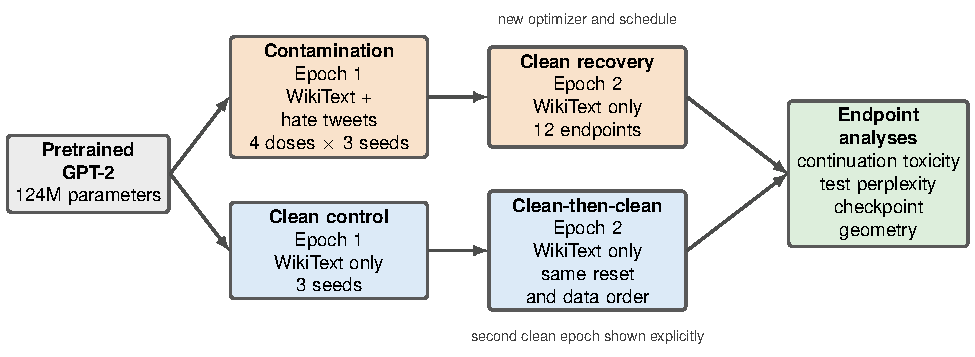
\includegraphics[width=\textwidth]{figures_v27/pipeline_v27.3.pdf}
\caption{Training and analysis pipeline. Every branch starts from pretrained GPT-2 and contains two one-epoch phases. Positive-dose models receive contamination followed by clean recovery; zero-dose controls receive clean training followed by a second clean epoch. Recovery and clean-then-clean use the same second-phase data order and optimizer reset. Endpoint evaluation re-scores final checkpoints without further training.}
\label{fig:pipeline}
\end{figure*}

\subsection{Matched-Threshold Temporal Analysis}
Let $B_s$ be the mean toxicity across evaluations of clean-control run $s$, and let $E_{d,s}$ be the mean of the final five contamination evaluations for dose $d$ and seed $s$. We compare acquisition and recovery at the shared halfway target
\begin{equation}
H_{d,s}=B_s+\frac{1}{2}(E_{d,s}-B_s).
\end{equation}
$B_s$ is an operational clean-control reference, not a measured pretrained score. Because no step-zero evaluation was recorded, a crossing in the first acquisition interval assumes that acquisition began below $H_{d,s}$.

We fit each acquisition series by nondecreasing isotonic least squares and each recovery series by nonincreasing isotonic least squares. This reduces dependence on isolated samples without imposing an exponential trajectory, but it assumes monotonicity and uses the complete recorded series. The evaluations immediately before and after the first fitted crossing define $A_s\in(L_{A,s},U_{A,s}]$ for acquisition and $R_s\in(L_{R,s},U_{R,s}]$ for recovery. If recovery does not cross by step 5,900, it is right-censored. The matched asymmetry ratio then satisfies
\begin{equation}
\rho_{50,s}=\frac{R_s}{A_s}>b_s\equiv\frac{L_{R,s}}{U_{A,s}}.
\end{equation}
We aggregate the paired seed-level lower bounds $b_s$. These intervals express the 50-step observation grid conditional on smoothing; they are not confidence intervals for a latent continuous process.

As a sensitivity analysis, we also fit each recovery series with an exponential curve anchored at $E_{d,s}$. Its half-life describes decay toward the fitted asymptote; it is not the time required to return halfway to the clean-control reference. We therefore treat the isotonic crossing analysis as primary and the exponential model as descriptive.

\subsection{Endpoint and Parameter-Space Analyses}
The endpoint evaluation addresses two weaknesses of the historical trajectories. For every final checkpoint, it generates five samples for each of the same 100 prompts using evaluation seeds shared across models, then scores only the newly generated continuation. It also computes token-weighted perplexity on the filtered WikiText-103 test set using a 128-token context and stride 64. A clean-then-clean control receives the same second WikiText epoch, data order, and optimizer reset as recovery. It nevertheless repeats its own first-phase clean sample, whereas each recovered model's first phase used a different WikiText sample mixed with tweets; this remaining corpus mismatch limits the control.

For the geometric analysis, $W_{\mathrm{pre}}$ denotes the pretrained weights, $W_{0,s}$ the first-phase clean control, $W_{d,s}$ the contaminated model, $W^R_{d,s}$ the recovered model, and $W^{CC}_{0,s}$ the clean-then-clean model. We use the full contamination displacement $C=W_{d,s}-W_{\mathrm{pre}}$, the toxicity-associated displacement $C_{\mathrm{tox}}=W_{d,s}-W_{0,s}$, the recovery displacement $R=W^R_{d,s}-W_{d,s}$, and the matched clean displacement $R_{\mathrm{cc}}=W^{CC}_{0,s}-W_{0,s}$. Cosines and projections describe endpoint movement; they do not identify a toxicity representation or reconstruct the training path. Finally, we evaluate $W^R_{d,s}-\alpha C_{\mathrm{tox}}$ for $\alpha\in\{0.5,1\}$ without retraining. The two values were not tuned.

\section{Results and Discussion}
\subsection{Rapid Acquisition and Partial Recovery}
Figure~\ref{fig:trajectories} shows that every tested dose produces a large increase in the measured score. Five-evaluation contamination endpoints average approximately 0.401, 0.412, 0.414, and 0.432 as dose increases. Recovery reduces these means to 0.264, 0.256, 0.261, and 0.244, but no recorded recovery evaluation returns to the pooled clean-control reference.

\begin{figure*}[t]
\centering
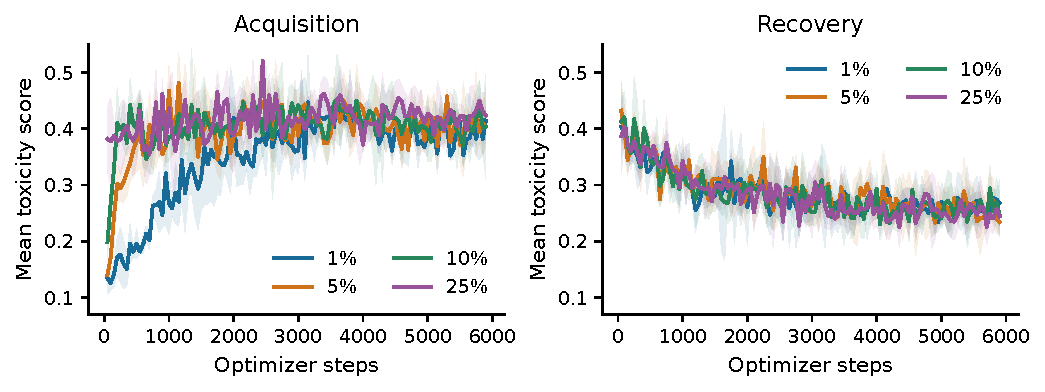
\includegraphics[width=\textwidth]{figures_v27/phase_trajectories.pdf}
\caption{Observed acquisition and recovery trajectories. Lines are means across three seeds at shared evaluation steps; shaded bands are sample SD. The grey line is the clean-then-clean control over the same second epoch. Scores include both prompt and continuation.}
\label{fig:trajectories}
\end{figure*}

Acquisition reaches the shared halfway target sooner than recovery in all twelve smoothed trajectories. The mean lower bounds on $\rho_{50}$ are $4.9\pm1.2$, $22.2\pm7.9$, $33.4\pm22.3$, and $60.3\pm13.9$ (Table~\ref{tab:matched}). Every per-run lower bound exceeds one, with a minimum of 3.74. Ten of twelve isotonic recovery curves cross the target within the recorded horizon; one 1\% run and one 10\% run remain censored. Because several ratios lack finite upper bounds and between-seed variation is large, the increasing lower bounds do not establish an increasing true ratio.

\begin{figure}[t]
\centering
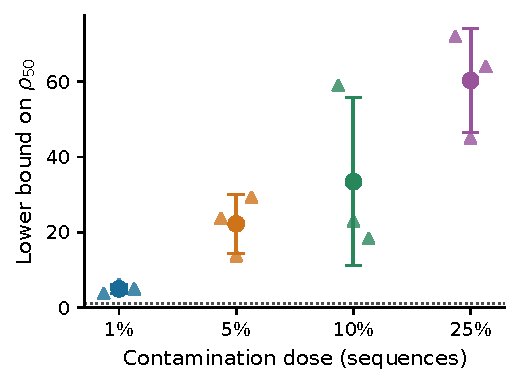
\includegraphics[width=\linewidth]{figures_v27/rho_matched.pdf}
\caption{Matched-threshold asymmetry. Triangles show each seed's lower bound $b_s$ on $\rho_{50,s}$; circles show their mean with sample SD. These are bounds on smoothed-curve crossing ratios, not point estimates or confidence intervals.}
\label{fig:rho}
\end{figure}

\begin{table*}[t]
\centering
\begin{tabular}{lcccc}
\toprule
Dose & Acquisition span & Isotonic crossings & Mean lower bound & Exponential crossings \\
 & (steps, all seeds) & (within horizon, /3) & $\overline b\pm\mathrm{SD}$ & (within horizon, /3) \\
\midrule
\inputrows{tables_v27/matched_summary.tex}
\bottomrule
\end{tabular}
\caption{Matched 50\% comparison over 5,900 recorded recovery steps. The acquisition span is the union of the three per-seed brackets. No censored run is discarded.}
\label{tab:matched}
\end{table*}

\subsection{Sensitivity to the Recovery Model}
Anchored exponential fits cross $H_{d,s}$ within 5,900 steps for eight of twelve runs, compared with ten isotonic crossings. Their half-lives range from $688\pm90$ to $788\pm392$ steps, with individual $R^2$ values from 0.40 to 0.66. These fits are useful summaries, but they provide limited evidence for an exact exponential process. Changing the endpoint averaging window, smoothing method, or clean reference changes some crossing classifications. The paired acquisition--recovery ordering persists in the tabulated analyses, whereas the exact ratio magnitude and number of completed recoveries remain analysis-dependent.

\subsection{Endpoint Re-Evaluation}
Continuation-only evaluation preserves the behavioral gap while removing prompt text from the classifier input. Recovered checkpoints score near 0.20 at every dose, roughly four times the mean clean-control score of 0.050 and well above the clean-then-clean mean of $0.049\pm0.009$ (Figure~\ref{fig:continuation}). The contamination-minus-recovery difference is positive in all twelve dose--seed pairs, and bootstrap intervals over prompts are above zero for every pair. This result shows that prompt content alone does not explain the endpoint difference; it does not retroactively convert the training-time trajectories into continuation-only measurements.

\begin{figure}[t]
\centering
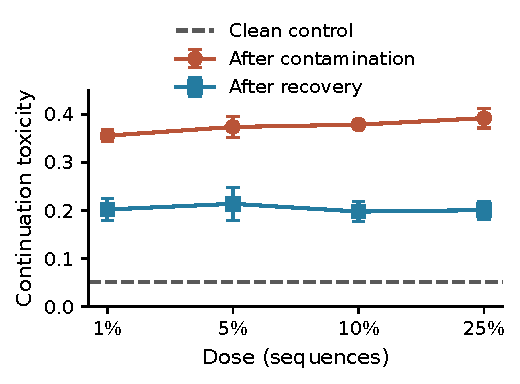
\includegraphics[width=\linewidth]{figures_v27/continuation_toxicity_by_dose.pdf}
\caption{Continuation-only Toxic-BERT scores at the final checkpoints. Error bars are sample SD across three data seeds.}
\label{fig:continuation}
\end{figure}

Contamination changes test perplexity modestly: relative to the cluster-trained clean controls, the largest increase is 0.53, or 2.2\%, at 25\% dose. Recovery lowers perplexity in every matched pair. Some of this improvement is ordinary continued training, as the clean-then-clean controls improve from 24.21 to 23.95. Thus recovery does not worsen perplexity on this filtered WikiText-103 evaluation, but this single in-domain metric does not establish general capability preservation.

\begin{table*}[t]
\centering\small
\setlength{\tabcolsep}{5pt}
\begin{tabular}{lcccccc}
\toprule
 & \multicolumn{3}{c}{Continuation-only toxicity} & \multicolumn{3}{c}{Test perplexity} \\
\cmidrule(lr){2-4}\cmidrule(lr){5-7}
Dose & Contam. & Recovered & C$-$R (paired) & Contam. & Recovered & R$-$C (paired) \\
\midrule
\inputrows{tables_v27/supplementary_summary.tex}
\midrule
Clean control & \multicolumn{3}{c}{$0.050\pm0.003$} & \multicolumn{3}{c}{$24.21\pm0.01$} \\
Clean-then-clean & \multicolumn{3}{c}{$0.049\pm0.009$} & \multicolumn{3}{c}{$23.95\pm0.04$} \\
Pretrained GPT-2 & \multicolumn{3}{c}{0.077} & \multicolumn{3}{c}{51.19} \\
\bottomrule
\end{tabular}
\caption{Endpoint re-evaluation: means and sample SD across three data seeds; differences are paired within seed. The clean perplexity reference uses the two cluster-trained clean controls.}
\label{tab:endpoint}
\end{table*}

\subsection{Parameter Movement and Task-Vector Negation}
Recovery does not retrace the full contamination displacement: the endpoint cosine $\cos(C,R)$ remains positive and falls from 0.64 to 0.55 as dose increases. Relative to $C_{\mathrm{tox}}$, recovery moves in the opposing direction and removes 32--33\% of that displacement by projection. The matched clean second epoch removes 17--19\%, showing that part of this movement also occurs under ordinary continued training. Recovery nevertheless removes 13--15 percentage points more in every dose--seed pair. At the same time, $\cos(R,R_{\mathrm{cc}})$ is 0.89--0.91, so most recovery movement follows the clean second epoch. These quantities describe a toxicity-associated direction that also contains differences in sampled WikiText rows; they do not isolate toxic information.

\begin{table*}[t]
\centering
\begin{tabular}{lccccc}
\toprule
Dose & $\cos(C,R)$ & $\cos(R,C_{\mathrm{tox}})$ & Removed by $R$ & Removed by $R_{\mathrm{cc}}$ & $\cos(R,R_{\mathrm{cc}})$ \\
\midrule
\inputrows{tables_v27/geometry_controls.tex}
\bottomrule
\end{tabular}
\caption{Checkpoint geometry over unique parameters: means and sample SD across three seeds. ``Removed'' is the projection $-\langle X,C_{\mathrm{tox}}\rangle/\|C_{\mathrm{tox}}\|^2$ for the indicated displacement $X$.}
\label{tab:geomctl}
\end{table*}

Subtracting $0.5C_{\mathrm{tox}}$ from each recovered model reduces continuation-only toxicity from about 0.20 to 0.055--0.066 in all twelve runs, removing 86--99\% of the gap above the clean-then-clean control. Test perplexity rises from about 23.7 to 24.1, an approximately 2\% cost. Subtracting the full displacement lowers the score further but raises perplexity by about 7\%. The edited models retain comparable bigram diversity, although Wikipedia-heading repetition increases. This intervention shows that movement along $C_{\mathrm{tox}}$ can causally change the measured behavior; because the direction contains other training differences, it does not uniquely locate toxicity.

\begin{table*}[t]
\centering\small
\begin{tabular}{lcccccc}
\toprule
 & \multicolumn{3}{c}{Continuation-only toxicity} & \multicolumn{3}{c}{Test perplexity} \\
\cmidrule(lr){2-4}\cmidrule(lr){5-7}
Dose & Recovered & $\alpha=0.5$ & $\alpha=1$ & Recovered & $\alpha=0.5$ & $\alpha=1$ \\
\midrule
\inputrows{tables_v27/negation.tex}
\midrule
Clean-then-clean & \multicolumn{3}{c}{$0.049\pm0.009$} & \multicolumn{3}{c}{$23.95\pm0.04$} \\
\bottomrule
\end{tabular}
\caption{Task-vector negation, $W^R_{d,s}-\alpha C_{\mathrm{tox}}$: means and sample SD across three seeds.}
\label{tab:negation}
\end{table*}


\section{Conclusion}
Under the tested GPT-2 protocol, toxicity acquisition reaches a seed-relative halfway target sooner than clean-data recovery. Explicit crossing intervals and censoring support that directional comparison without turning incomplete observations into precise ratios. No recorded recovery evaluation returns to the clean-control reference, and continuation-only endpoint scoring preserves the residual gap. Recovery also opposes only part of the toxicity-associated parameter displacement; a direct edit along that direction substantially reduces the measured score, with a modest in-domain perplexity cost.

These findings describe a controlled proof of concept, not a universal law of safety recovery. They motivate longer recovery schedules, domain-matched controls, additional toxicity measures, and experiments with larger aligned models before drawing broader conclusions about safety or unlearning.

\section*{Limitations}
The study uses one small unaligned model, one toxicity classifier, one fixed prompt set, three data seeds, and a one-epoch recovery schedule whose learning rate decays toward zero. Toxic-BERT is an imperfect proxy for harmful language: Appendix~\ref{app:data} includes a clearly anti-immigrant continuation that it scores only 0.005. Because the main outcomes are classifier scores, the results establish changes in this measurement rather than complete changes in human-judged toxicity. Historical trajectories score prompt and continuation together using one unseeded generation per prompt; continuation-only scores are available only at final checkpoints. The clean reference averages an evolving training run rather than measuring the pretrained model at step zero. Isotonic smoothing, endpoint averaging, and the chosen reference can affect individual crossings, and three seeds do not provide precise uncertainty estimates.

Data construction also limits interpretation. Mixing hate-labeled tweets into predominantly Wikipedia text changes domain and linguistic style along with harmful content. A benign, domain-matched tweet control is needed to isolate toxicity from ordinary adaptation to short, informal text. Toxic examples repeat, the nominal sequence dose differs from token exposure, validation rows overlap training sources, and recovered models do not see exactly the same first-phase WikiText rows as clean-then-clean controls. One clean control was trained in a different software environment. Finally, $C_{\mathrm{tox}}$ is toxicity-associated rather than toxicity-specific, and task-vector negation uses a matched clean checkpoint that would not generally be available for an uncontrolled contaminated model.

\section*{AI Disclosure and Reflection}
AI assistants -- Gemini 3.1 Pro, GPT 6 Astra, and Claude Opus 5.5 -- supported code organization, Slurm scripts, quantitative auditing, and revisions to the paper. Gemini assisted with geometric-analysis boilerplate and migration from Colab to Slurm. Claude Code assisted with checking claims against code and logs, implementing endpoint re-evaluation, regenerating figures, and drafting corrections. The authors designed the experiments, selected the analyses, verified the reported results, and remain responsible for every claim. The tools were most useful for debugging and consistency checks, as well as Git management; their proposed wording and interpretations required substantial human review, particularly where fluent language overstated what the experiments established.
